% --------------------------------------------------------------
% This is all preamble stuff that you don't have to worry about.
% Head down to where it says "Start here"
% --------------------------------------------------------------
 
\documentclass[12pt]{article}
 
\usepackage[margin=1in]{geometry} 
\usepackage{amsmath,amsthm,amssymb}
\usepackage{mathtools}
\usepackage{graphicx}
\usepackage{tikz}
\usepackage{subfig}
\usepackage{tcolorbox}
 
\newcommand{\N}{\mathbb{N}}
\newcommand{\Z}{\mathbb{Z}}
 
\newenvironment{theorem}[2][Theorem]{\begin{trivlist}
\item[\hskip \labelsep {\bfseries #1}\hskip \labelsep {\bfseries #2.}]}{\end{trivlist}}
\newenvironment{lemma}[2][Lemma]{\begin{trivlist}
\item[\hskip \labelsep {\bfseries #1}\hskip \labelsep {\bfseries #2.}]}{\end{trivlist}}
\newenvironment{exercise}[2][Exercise]{\begin{trivlist}
\item[\hskip \labelsep {\bfseries #1}\hskip \labelsep {\bfseries #2.}]}{\end{trivlist}}
\newenvironment{reflection}[2][Reflection]{\begin{trivlist}
\item[\hskip \labelsep {\bfseries #1}\hskip \labelsep {\bfseries #2.}]}{\end{trivlist}}
\newenvironment{proposition}[2][Proposition]{\begin{trivlist}
\item[\hskip \labelsep {\bfseries #1}\hskip \labelsep {\bfseries #2.}]}{\end{trivlist}}
\newenvironment{corollary}[2][Corollary]{\begin{trivlist}
\item[\hskip \labelsep {\bfseries #1}\hskip \labelsep {\bfseries #2.}]}{\end{trivlist}}
\newenvironment{question}[2][Question]{\kern10pt \begin{trivlist}
\begin{tcolorbox}
\item[\hskip \labelsep {\bfseries #1}\hskip \labelsep {\bfseries #2.}]}
{\end{tcolorbox} \end{trivlist}}
 
\newcommand\mytodo[1]{\textcolor{red}{#1}}

\newcommand*{\answer}{%
  \par
  \kern1pt
  \begingroup
    \centering
    \raisebox{.2\baselineskip}{%
      \textcolor{gray}{
	    \rule{.6667\linewidth}{.1pt}%
      }
    }%
    \par
  \kern8pt
  \endgroup
}

\begin{document}
 
\graphicspath{ {img/} }
% --------------------------------------------------------------
%                         Start here
% --------------------------------------------------------------
 
\renewcommand{\qedsymbol}{\filledbox}
 
\title{Machine Learning, Advanced Course (DD2434)\\
		Assignment 2}
\author{Martin Hwasser, hwasser@kth.se}
 
\maketitle

\begin{question}{1}

In which pairs is one value larger than the other?
\end{question}
$$p(t^1 \vert d^1) < p(t^1)$$
$$p(d^1 \vert t^0) > p(d^1)$$
$$p(h^1 \vert e^1, f^1) > p(h^1 \vert e^1)$$
$$p(c^1 \vert h^0) < p(c^1)$$

\begin{question}{2}
Which pairs are equal?
\end{question}
$$p(c^1 \vert f^0) = p(c^1)$$
$$p(d^1 \vert h^1, e^0) = p(d^1 \vert h^1)$$
$$p(c^1 \vert h^0, f^0) = p(c^1 \vert h^0)$$

\begin{question}{3}
Which pairs are incomparable (i.e., the two values can not be compared based on the information available in the DAG.)
\end{question}
\begin{center}
$p(d^1 \vert e^1, f^0, w^1)$ and $p(d^1 \vert e^1, f^0)$
\\
$p(t^1 \vert w^1, f^0)$ and $p(t^1 \vert w^0)$
\end{center}

\begin{question}{6}
Provide data generated using at least three different sets of categorical dice distributions – what does it look like for all unbiased dice, i.e., uniform distributions, for example, or if some are biased in the same way, or if some are unbiased and there are two different groups of biased dice.
\end{question}

Figure \ref{casino_fair} shows the distribution of outcomes when the dices of both the casino and the players have a uniform distribution.

Figure \ref{casino_c_unfair} shows the distribution of outcomes when players have fair dices, but the primed tables have a distribution like $p(1) = \frac{5}{10}$ and $p(1>) = \frac{1}{5}$.

Figure \ref{casino_p_unfair} shows the distribution of outcomes when the casino have biased dices like in \ref{casino_c_unfair}, but the players also have a biased distribution $p(<6) = \frac{1}{7}$ and $p(6) = \frac{2}{7}$.

\begin{figure}
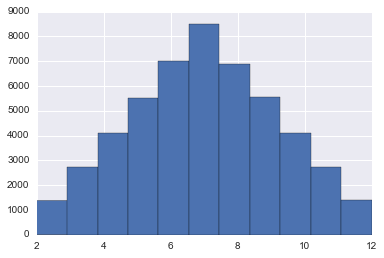
\includegraphics[]{casino_fair}
\centering
\caption{Both casino and player have fair dices.}
\label{casino_fair}
\end{figure}

\begin{figure}
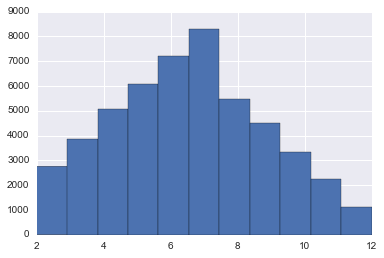
\includegraphics[]{casino_c_unfair}
\centering
\caption{The casino has unfair dices on certain tables.}
\label{casino_c_unfair}
\end{figure}

\begin{figure}
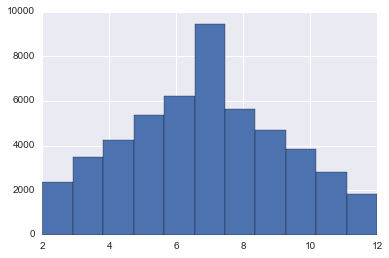
\includegraphics[]{casino_p_unfair}
\centering
\caption{Both the casino and the players have unfair dices.}
\label{casino_p_unfair}
\end{figure}
% --------------------------------------------------------------
%     You don't have to mess with anything below this line.
% --------------------------------------------------------------
 
\end{document}
